% Author: Max Melching (2025)
% Heavily inspired by Figs. 5.49, 5.50 in Griffiths Electrodynamics (4th edition)
\documentclass[border=3pt,tikz]{standalone}

\usepackage{physics}
\usepackage{tikz}
\usepackage{tikz-3dplot}
\usepackage[outline]{contour} % glow around text
\usepackage{xcolor}

\usepackage{newtxmath}
\usepackage{tgpagella}

\colorlet{mygreen}{green!60!black}
\colorlet{myred}{red!90!black}
\colorlet{myblue}{blue!80!black}


\usetikzlibrary{calc, 3d, arrows.meta, decorations.markings, decorations.pathreplacing}


\tikzset{
    >={Stealth[inset=0,angle'=27]},
    surface/.style={
        left color=gray!10,
        right color=gray!80,
    },
    labelarrow/.style={
        ->,
        thick,
        myblue,
    },
}



% -- Quick command for custom rectangle
% \def\rect#1#2{(#1,#2) --++ (2,1) --++ (1,-1) --++ (-2,-1) -- cycle}
% \def\rect#1#2{(#1,#2) --++ (2,0.7) --++ (1,-0.3) --++ (-2,-0.7) -- cycle}
\def\rect#1#2{%
    (#1,#2) --++ (2,0.7) --++ (1,-0.3) --++ (-2,-0.7) --++ (-1,0.3)% Upper rectangle
    --++ (0,-0.12) --++ (1,-0.3) --++ (0,0.12) --++ (-1,0.3)% Left lower side
    % --++ (1,-0.3) --++ (2,0.7) --++ (0,-0.12) --++ (-2,-0.7) ++ (0,0.12)% Right lower side
    --++ (0,-0.12) --++ (1,-0.3) --++ (2,0.7) --++ (0,0.12) --++ (-2,-0.7) ++ (0,-0.12)% Right lower side
}


\begin{document}


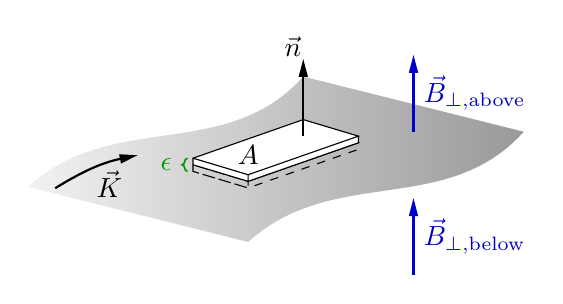
\begin{tikzpicture}[scale=0.7]
    % \draw[] (0,0) to[out=42,in=-90-42] (5,2) -- (9,1) to[out=-90-42,in=42] (4,-1) -- cycle;
    \shade[surface] (0,0) to[out=42,in=-90-42] (5,2) -- (9,1) to[out=-90-42,in=42] (4,-1) -- cycle;

    \draw[->, thick, shift={(0.5,-0.025)}] (0,0) to[bend left=10] (1.5,0.6) node[below left=2] {$\vec{K}$};  % With shift to easily match curvature of surface


    \def\Rx{3}
    \def\Ry{0.4}


    \draw[dashed] \rect{\Rx}{\Ry};
    \draw[fill=white] \rect{\Rx}{\Ry+0.12};
    
    % \node at (4.2,0.6) {$A$};
    \node at ({\Rx + 0.5 + 0.5},{\Ry + 0 + 0.175}) {$A$};
    \draw[->, thick] (\Rx,\Ry) ++ (0.5,0) ++ (1.5,0.525) --++ (0,1.4) node[above left=-3] {$\vec{n}$};
    % \draw[->, thick] (\Rx,\Ry) ++ (0.5,0.12) ++ (1.5,0.525) --++ (0,1.4) node[above left=-3] {$\vec{n}$};
    % \draw[thick, dotted] (\Rx,\Ry) ++ (0.5,0.12) ++ (1.5,0.525) --++ (0,-\Ry);

    \draw[
        mygreen,
        semithick,
        decorate,
        decoration={
            brace,
            amplitude=2pt,
            raise=2pt,
            mirror,
        },
    ]  (\Rx, \Ry) ++ (0,0.12) --++ (0,-0.12*2) node[midway,left=4] {$\epsilon$};


    % \draw[fill,myblue] (7,0.7) circle(0.07);
    \draw[labelarrow] (7,-1.6) --++ (0,1.4) node[midway,right] {$\vec{B}_{\perp, \mathrm{below}}$};
    \draw[labelarrow] (7,1) --++ (0,1.4) node[midway,right] {$\vec{B}_{\perp, \text{above}}$};
\end{tikzpicture}



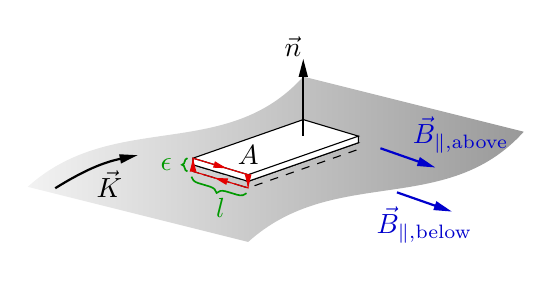
\begin{tikzpicture}[scale=0.7]
    % \draw[] (0,0) to[out=42,in=-90-42] (5,2) -- (9,1) to[out=-90-42,in=42] (4,-1) -- cycle;
    \shade[surface] (0,0) to[out=42,in=-90-42] (5,2) -- (9,1) to[out=-90-42,in=42] (4,-1) -- cycle;

    \draw[->, thick, shift={(0.5,-0.025)}] (0,0) to[bend left=10] (1.5,0.6) node[below left=2] {$\vec{K}$};  % With shift to easily match curvature of surface


    \def\Rx{3}
    \def\Ry{0.4}


    \draw[dashed] \rect{\Rx}{\Ry};
    \draw[fill=white] \rect{\Rx}{\Ry+0.12};

    % \node at (4.2,0.6) {$A$};
    \node at ({\Rx + 0.5 + 0.5},{\Ry + 0 + 0.175}) {$A$};
    \draw[->, thick] (\Rx,\Ry) ++ (0.5,0) ++ (1.5,0.525) --++ (0,1.4) node[above left=-3] {$\vec{n}$};

    % \draw[
    %     <-,
    %     thick,
    %     mygreen,
    % ] (\Rx, \Ry) ++ (0,0.12) ++ (-0.25,0) --++ (0,1);
    
    % \draw[
    %     <-,
    %     thick,
    %     mygreen,
    % ] (\Rx, \Ry) ++ (0,-0.12) ++ (-0.25,0) --++ (0,-1);

    % \draw[mygreen, thin] (\Rx, \Ry) ++ (0,0.12) ++ (-0.05,0) --++ (-0.4,0);
    % \draw[mygreen, thin] (\Rx, \Ry) ++ (0,-0.12) ++ (-0.05,0) --++ (-0.4,0);
    
    % \node[mygreen] at ({\Rx - 0.05 - 0.2}, \Ry) {$\epsilon$};

    \draw[
        mygreen,
        semithick,
        decorate,
        decoration={
            brace,
            amplitude=2pt,
            raise=2pt,
            mirror,
        },
    ]  (\Rx, \Ry) ++ (0,0.12) --++ (0,-0.12*2) node[midway,left=4] {$\epsilon$};


    \draw[
        myred,
        postaction=decorate,
        decoration={
            markings,
            mark=between positions 0.045 and 1 step 0.25 with \arrow{>}
        },
    % ] (\Rx,\Ry) ++ (0,0.12) --++ (1,-0.3) --++ (0,-0.12*2) --++ (-1,0.3) --++ (0,2*0.12);
    ] (\Rx,\Ry) --++ (0,0.12) --++ (1,-0.3) --++ (0,-0.12*2) --++ (-1,0.3) --++ (0,0.12);  % Testing with arrows -> this one better

    \draw[
        mygreen,
        semithick,
        decorate,
        decoration={
            brace,
            amplitude=3pt,
            raise=2pt,
            mirror,
        },
    ] (\Rx,\Ry) ++ (0,-0.12) --++ (1,-0.3) node[midway,below=3]{$l$};
    

    % \draw[fill,myblue] (7.7,0.9) circle(0.07);
    % \draw[labelarrow] (7.7,0.6) --++ (-1,-0.35) node[midway,below right] {$\vec{B}_{\parallel, \mathrm{below}}$};
    % \draw[labelarrow] (7.7,1.2) --++ (-1,-0.35) node[midway,above left=1] {$\vec{B}_{\parallel, \text{above}}$};
    % -- Same ratio as the edge with (2,0.7), which is edge we are trying to be parallel to
    
    \draw[labelarrow] (6.7,-0.1) --++ (1,-0.35) node[midway,below=-2] {$\vec{B}_{\parallel, \mathrm{below}}$};
    \draw[labelarrow] (6.4,0.7) --++ (1,-0.35) node[midway,above right=-2] {$\vec{B}_{\parallel, \text{above}}$};
\end{tikzpicture}



\end{document}